%pdflatex -halt-on-error -aux-directory=tmp -output-directory=tmp rapport.tex%

\documentclass{article}
\usepackage{amsmath}
\usepackage[utf8]{inputenc}
\usepackage[T1]{fontenc}
\usepackage{graphicx}
\usepackage{hyperref}
\usepackage[francais]{babel}
\usepackage{listings}
\usepackage{xcolor}

\definecolor{codegreen}{rgb}{0,0.6,0}
\definecolor{codegray}{rgb}{0.5,0.5,0.5}
\definecolor{codepurple}{rgb}{0.58,0,0.82}
\definecolor{backcolour}{rgb}{0.95,0.95,0.92}

\lstdefinestyle{mystyle}{
    language=python,
    backgroundcolor=\color{backcolour},   
    commentstyle=\color{codegreen},
    keywordstyle=\color{magenta},
    numberstyle=\tiny\color{codegray},
    stringstyle=\color{codepurple},
    basicstyle=\ttfamily\footnotesize,
    breakatwhitespace=false,         
    breaklines=true,                 
    captionpos=b,                    
    keepspaces=true,                 
    numbers=left,                    
    numbersep=5pt,                  
    showspaces=false,                
    showstringspaces=false,
    showtabs=false,                  
    tabsize=2
}

\lstset{style=mystyle}

\title{Système d'exploitation}
\author{Wassim SAIDANE}
\date{Mise à jour 19/01/2021}

\begin{document}
    \pagenumbering{gobble}
    \maketitle
    \tableofcontents
    \newpage
    \pagenumbering{arabic}
    \section{Présentation des systèmes d'exploitation}
    \subsection{Un ordinateur}
    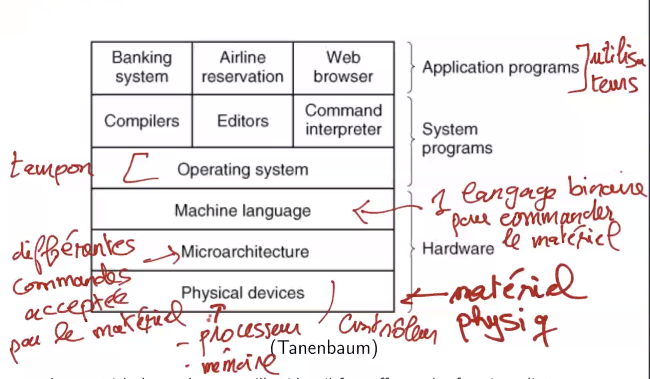
\includegraphics{1.PNG}
    Le matériel n'est qu'une coquille vide : il faut affecter les fonctionnalités
    \subsection{Un OS}
    Le logiciel qui cache la complexité de l'architecture matérielle et la rend facilement exploitable. \\
    Du point du vue utilisateur on ne veut pas savoir toutes les informations sur le matériel utilisé. \\
    Un OS donne aux développeurs une base (/bin) et rend les choses simples, uniformes et cohérente (/media) \\
    OS = machine virtuelle plus facile à programmer et gestionnaire de ressources. \\
    Cette machine virteulle contrôle les accés aux ressources, uniformise les accès et si possible simplifie l'accés. \\
    Le système d'exploitation est une machine virtuelle car on n'a pas à se soucier de comment invoquer les commandes des périphiques. \\
    Il est également un un gestionnaire de ressources : Gestion d'accès aux différents péripériques. \\
    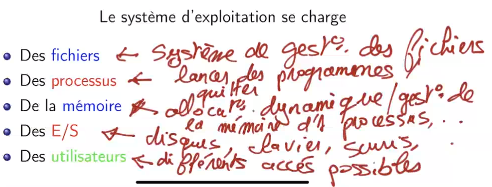
\includegraphics{2.PNG}
    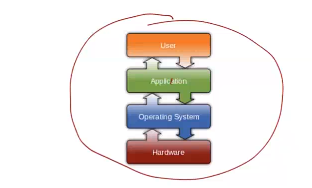
\includegraphics{3.PNG} \\
    Un OS ce n'est pas : \\
    - L'interpète de commandes \\
    - L'interface graphique \\
    - Les utilitaires \\
    - Le BIOS \\
    \newpage
    Un OS c'est : \\ 
    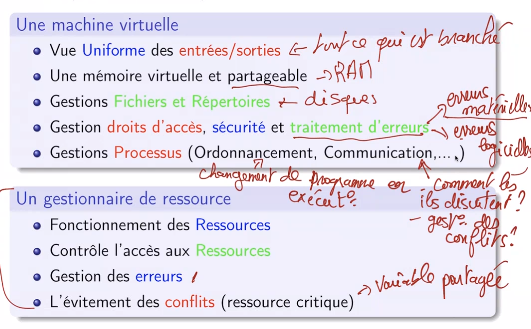
\includegraphics{4.PNG}
    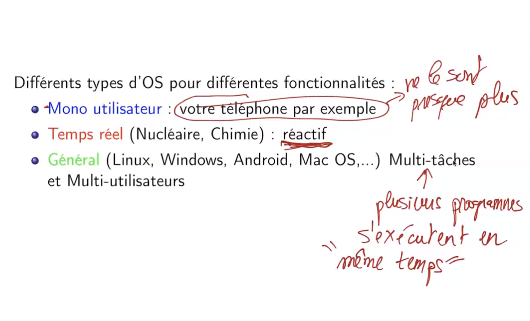
\includegraphics{5.PNG} \\
    \\
    \newpage
    Les programmes en exécution sont encapsulés dans des processus : \\
    - Gestion multi-programmation \\
    - Gestion des communications entre programmes \\ 
    - Gestion des attentes de réponse des programmes \\
    - Droits associés aux restrictions fixés aux utilisateurs \\
    \\
    Les programmes en exécution sont encapsulés dans des processus \\
    - Gestion multi-programmation \\
    - Gestion des communications entre programmes \\
    - Gestion des attentes de réponse des programmes \\
    - Droits associés aux restrictions fixés aux utilisateurs \\
    \\
    (Systèmes de) Fichiers \\
    - Les données stockées dans des objetsappelés fichiers et on s'abstrait des disque.\\
    - Gestion des droits d'accès aux fichiers. \\
    \\
    Mémoire  \\
    - Gestion de la mémoire d'exéctuin des programmes par espaces d'adressage. \\
    - Mémoire transformée en mémoire virtuelle. \\
    \\
    Un ensemble de fonctions systèmes avex des super-droits et une sémentique d'appel particulière appelée appels systèmes. \\
    - Linterpréteur Shell est l'exemple type utilisant beaucoup les appels systèmes. 
    \section{Principe des appels systèmes et interface POSIX}
    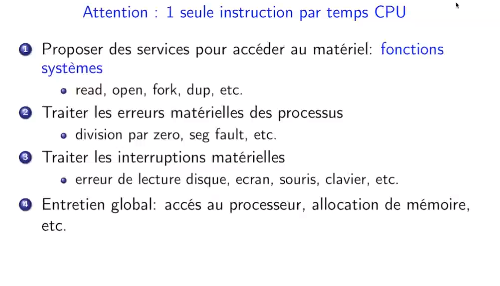
\includegraphics{6.PNG}
    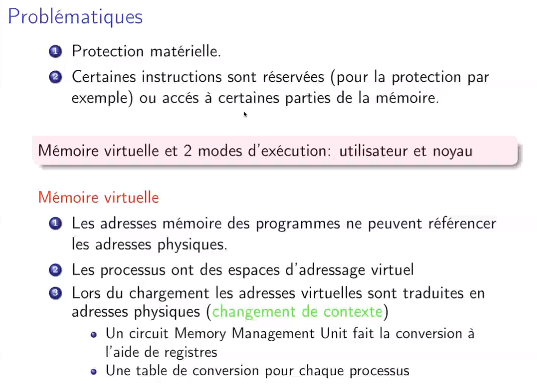
\includegraphics{7.PNG}
    
\includegraphics{8.PNG}
    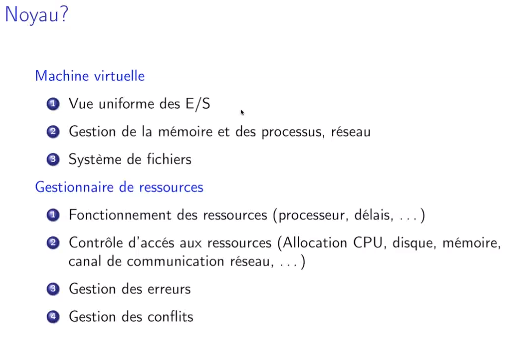
\includegraphics{9.PNG}
    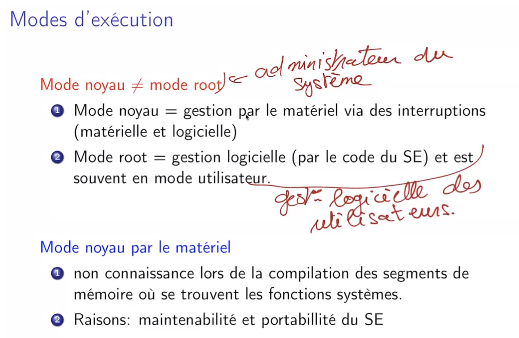
\includegraphics{10.PNG}
    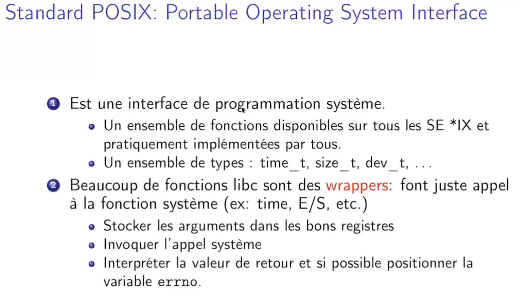
\includegraphics{11.PNG}
    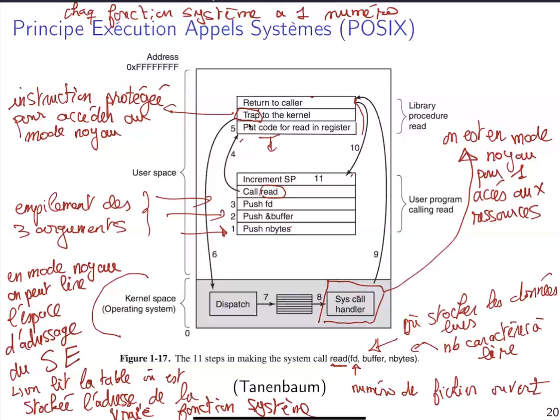
\includegraphics{12.PNG}
    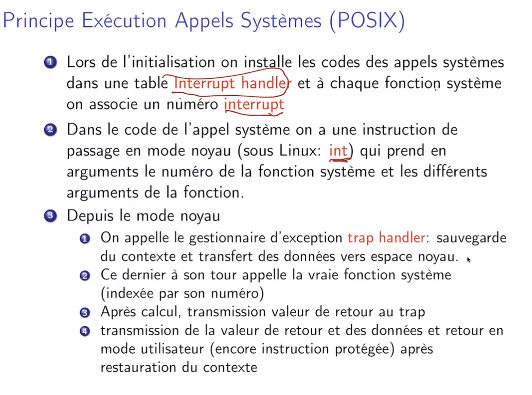
\includegraphics{13.PNG}
    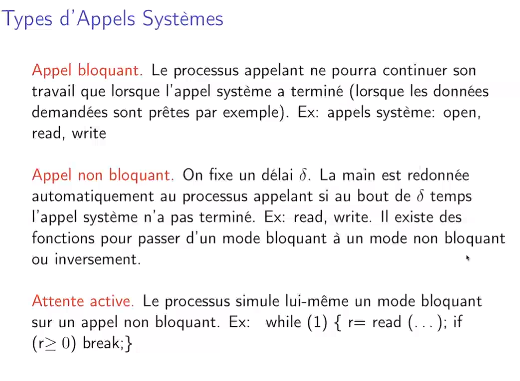
\includegraphics{14.PNG}
    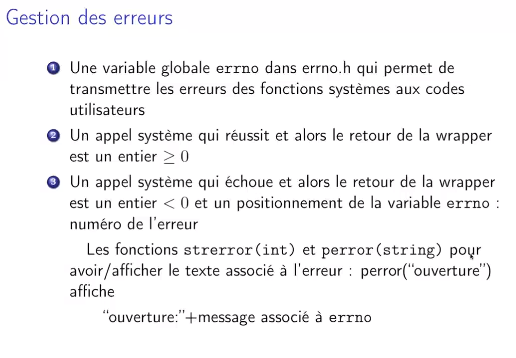
\includegraphics{15.PNG}
    \section{Gestion de la mémoire}
    \section{Gestion des processus}
    \section{Gestion des fichiers}
    
\end{document}
